
To test our generative-evaluative learning architecture we compared the grasp it proposes to the grasp proposed by the generative learner alone. Since \citet{kopicki2015ijrr} showed a 77.7\% success rate with the original generative algorithm we generated a new test set that contained both more challenging objects and placed them in challenging poses. The difficulty single-view grasping with a depth camera depends greatly on the pose of the object relative to the camera. The set comprised 40 test objects (Figure~\ref{fig:real-objects}) and another six training objects. The training objects were used by the human to demonstrate ten example grasps (Figure~\ref{fig:generative-training}). The 40 test objects were used to generate 49 object-pose pairs. From the 40 objects, 35 belonged to object classes in the simulation dataset, while the remaining five do not. 

\begin{figure}
  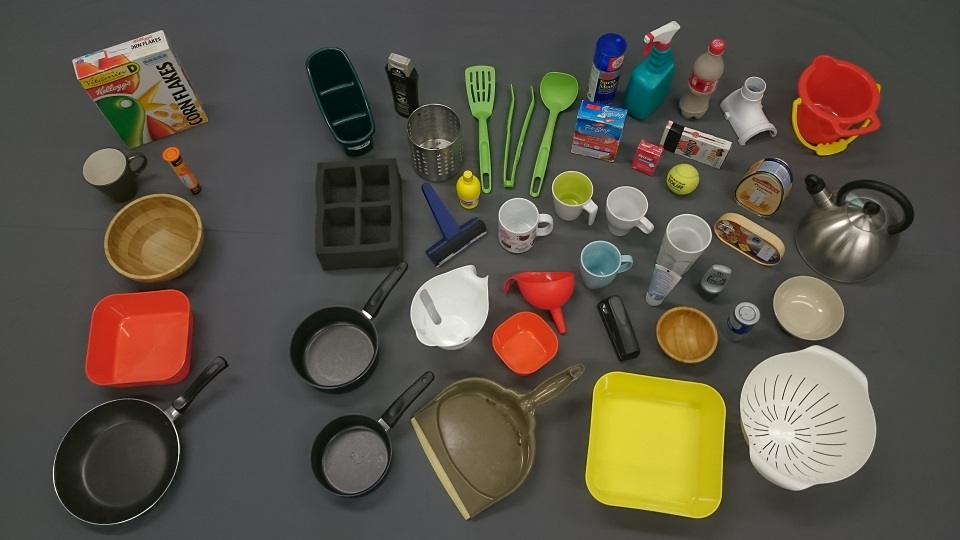
\includegraphics[width=\linewidth]{images/objects.jpg}
  \caption{The real objects. The training objects are on the left, testing objects are on the right.}
  \label{fig:real-objects}
\end{figure}

A pure generative model architecture (GM) and the generative-evaluative architecture (GEA) were evaluated using a paired trials methodology. Each was presented with the same object-pose combinations. Each architecture generated a ranked list of grasps, and the highest ranked grasp was executed. The highest-ranked grasp based on the predicted success probability of the network is performed on each scene. A grasp was deemed successful if, when lifted for five seconds, the object then remained stable in the hand for a further five seconds before being automatically released. The success rate for GM was 57.1\% and for GEA it was 77.6\%. The successes and failures for each method were recorded and are summarised in Table~\ref{tab:robot-results}. A two-tailed McNemar test, for the difference between success rates for paired comparison data, was performed and the difference between the two algorithms has a $p$-value of 0.0442, and so is statistically significant.
\begin{table}
\begin{center}
\caption{Results of the real robot paired comparison trial.}
\begin{tabular}{|c|c|c|c|}  \hline 
          &                & \multicolumn{2}{ c |}{ GM} \\ \hline
          &                & \# succs & \# fails  \\  \hline
 GEA  & \# succs &  23 &  15  \\
          & \# fails    &  5   &   6   \\ \hline
\end{tabular}
\end{center}
\label{tab:robot-results}
\end{table}
A selection of grasps where the two methods performed differently are shown.
%Training parameters for network. Training of example grasps for learning from demonstration. Creation of real test data set. Paired comparisons methodology with vanilla LFD algorithm (pose + object + camera view).
%
%The actual grasping tests have been performed on the real robot. 